
%\documentstyle[epsf,twocolumn]{jarticle}       %LaTeX2e仕様
\documentclass[twocolumn]{jarticle}     %pLaTeX2e仕様(platex.exeの場合)
% \documentclass[onecolumn]{ujarticle}   %pLaTeX2e仕様(uplatex.exeの場合)
%%%%%%%%%%%%%%%%%%%%%%%%%%%%%%%%%%%%%%%%%%%%%%%%%%%%%%%%%%%%%%
%%
%%  基本バージョン
%%
%%%%%%%%%%%%%%%%%%%%%%%%%%%%%%%%%%%%%%%%%%%%%%%%%%%%%%%%%%%%%%%%
\setlength{\topmargin}{-45pt}
%\setlength{\oddsidemargin}{0cm}
\setlength{\oddsidemargin}{-7.5mm}
%\setlength{\evensidemargin}{0cm}
\setlength{\textheight}{24.1cm}
%setlength{\textheight}{25cm}
\setlength{\textwidth}{17.4cm}
%\setlength{\textwidth}{172mm}
\setlength{\columnsep}{11mm}

%\kanjiskip=.07zw plus.5pt minus.5pt


% 【節が変わるごとに (1.1)(1.2) … (2.1)(2.2) と数式番号をつけるとき】
%\makeatletter
%\renewcommand{\theequation}{%
%\thesection.\arabic{equation}} %\@addtoreset{equation}{section}
%\makeatother

%\renewcommand{\arraystretch}{0.95} 行間の設定
%%%%%%%%%%%%%%%%%%%%%%%%%%%%%%%%%%%%%%%%%%%%%%%%%%%%%%%%
%\usepackage{graphicx}   %pLaTeX2e仕様(\documentstyle ->\documentclass)
\usepackage[dvipdfmx]{graphicx}
\usepackage{subcaption}
\usepackage{multirow}
\usepackage{amsmath}
\usepackage{url}
\usepackage{ulem}
\usepackage{algorithm}
\usepackage{algorithmic}
\usepackage{listings} %,jlisting} %日本語のコメントアウトをする場合jlistingが必要
%ここからソースコードの表示に関する設定
\lstset{
  basicstyle={\ttfamily},
  identifierstyle={\small},
  commentstyle={\smallitshape},
  keywordstyle={\small\bfseries},
  ndkeywordstyle={\small},
  stringstyle={\small\ttfamily},
  frame={tb},
  breaklines=true,
  columns=[l]{fullflexible},
  numbers=left,
  xrightmargin=0zw,
  xleftmargin=3zw,
  numberstyle={\scriptsize},
  stepnumber=1,
  numbersep=1zw,
  lineskip=-0.5ex
}
\newcommand{\argmax}{\mathop{\rm arg~max}\limits}
\newcommand{\argmin}{\mathop{\rm arg~min}\limits}

%%%%%%%%%%%%%%%%%%%%%%%%%%%%%%%%%%%%%%%%%%%%%%%%%%%%%%%%
\begin{document}

	%bibtex用の設定
	%\bibliographystyle{ujarticle}

	\twocolumn[
		\noindent
		\hspace{1em}
		2021 年 4 月 9 日
		ゼミ資料
		\hfill
		M1 杉山 竜弥
		\vspace{2mm}

		\hrule
		\begin{center}
			{\Large \bf 進捗報告}
		\end{center}
		\hrule
		\vspace{9mm}
	]

\section{今週やったこと}
\begin{itemize}
  \item TDGA + DARTS の追加実験
  \item LSTM の動作確認
\end{itemize}


\section{実験1}

\begin{table}[tb]
  \begin{center}
    \caption{モデルの設定}
    \begin{tabular}{|c|c|} \hline
      base model & VGG19 \\ \hline
      Optim($w$) & SGD(lr=0.001, momentum=0.9) \\ \hline
      Optim($\alpha$) & Adam(lr=0.001, $\beta$=(0.5, 0.999)) \\ \hline
      Loss & Cross Entropy Loss \\ \hline
      dataset & cifar10 \\ \hline
      pretrain & true \\ \hline
      batch size & 64 \\ \hline
      train size & 25000 \\ \hline
      valid size & 25000 \\ \hline
    \end{tabular}
    \label{tab:setting}
  \end{center}
\end{table}

TDGA + DARTS の試行回数が少なかったため, 追加実験を行った.

表 \ref{tab:setting} にモデルの設定を示す.
図 \ref{fig:acc} に合計 3 回試行した TDGA の実験結果を示した.
1 回試行のときと大きくは変わらず, TDGA のみによる探索が安定して, 精度の向上がみられる.
しかし全体の改善は, 0.1 \% 程度であまり改善はなされていない.

\begin{figure}[tb]
  \begin{center}
    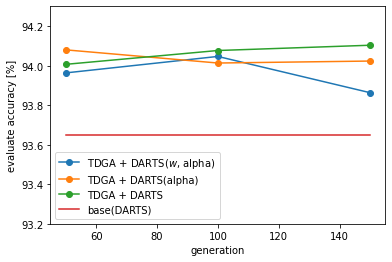
\includegraphics[clip,width=75mm]{3com.png}
    \caption{3 回試行の結果}
    \label{fig:acc}
  \end{center}
\end{figure}


\section{実験2}

\begin{table}[tb]
  \begin{center}
    \caption{LSTMの設定}
    \begin{tabular}{|c|c|} \hline
      component & LSTM + Linear \\ \hline
      Optim & Adam(lr=0.01, $\beta$=(0.5, 0.999)) \\ \hline
      Loss & MSE \\ \hline
      hidden size & 5 dim \\ \hline
      data length & train=100, test=50 \\ \hline
      data size & train=10000, test=1000 \\ \hline
      epoch & 250 \\ \hline
      batch size & 100 \\ \hline
    \end{tabular}
    \label{tab:setting_lstm}
  \end{center}
\end{table}
% \begin{table}[tb]
%   \begin{center}
%     \caption{結果}
%     \begin{tabular}{|c|c|c|} \hline
%       タイプ & accuracy(\%) & alpha \# \\ \hline\hline
%       A & 93.71 & 17 * 17 \\ \hline
%       B & 93.74 & 17 * 2 \\ \hline
%       C & 93.80 & 17 * 3 - 1 \\ \hline
%     \end{tabular}
%     \label{tab:result}
%   \end{center}
% \end{table}

実験1 のアーキテクチャ探索でネックとなる, アーキテクチャの学習や評価を RNN の利用によって,
処理を代替的に予測して, 探索時間を削減する実験の第一歩として, まず LSTM の知識や動作を確認した.


表 \ref{tab:setting_lstm} に LSTM の設定を示した.
時系列長 100 のデータから次の値を予測するように学習し,
テストでは時系列長 50 のデータから再帰的に 50 ステップ先まで予測した.

図 \ref{fig:lstm}, \ref{fig:lstm2} に $\sin$ 波などから作成したデータセットのテストの結果を示す.
値域が小さい周期関数は, ある程度高い精度で予測できることが分かった.

また Optimizer は SGD よりも Adam が格段に学習が早いので, Adam を採用する.


\begin{figure}[tb]
  \begin{center}
    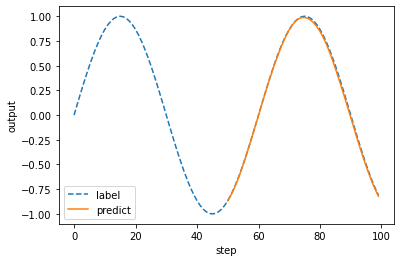
\includegraphics[clip,width=75mm]{lstm_sin.png}
    \caption{LSTM の動作確認 : sin 波}
    \label{fig:lstm}
  \end{center}
\end{figure}
\begin{figure}[tb]
  \begin{center}
    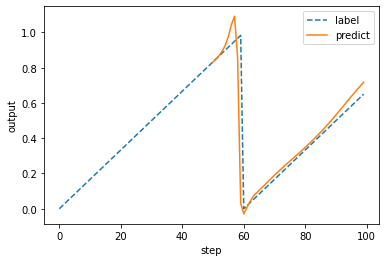
\includegraphics[clip,width=75mm]{lstm.png}
    \caption{LSTM の動作確認 : ノコギリ?}
    \label{fig:lstm2}
  \end{center}
\end{figure}

問題点
\begin{itemize}
  \item $y = x$ など関数の値が大きすぎるとうまく学習できない (loss が不安定になるのが原因?)
  \item データ数が足りないので増やす
\end{itemize}

\section{今後の予定}
% なんとなくなんかの勉強をするとかではなく具体的に
\begin{itemize}
  \item データセットを作成する (データは現在増強中)
  \item LSTM で実験する
\end{itemize}

% 参考文献リスト
\bibliographystyle{unsrt}
\bibliography{ref}
\end{document}
